\documentclass{article}
\usepackage[utf8]{inputenc}
\usepackage{floatrow}
\usepackage{amsmath}

\addtolength{\oddsidemargin}{-.875in}
\addtolength{\evensidemargin}{-.875in}
\addtolength{\textwidth}{1.75in}

\addtolength{\topmargin}{-0.875in}
\addtolength{\textheight}{1.75in}

% -------------------------------------------------------------
% ------------------- Title section ---------------------------
% -------------------------------------------------------------

\title{PHY 153 Final Project}
\author{Henry Shi}
\date{Fall 2019 (make-up in Spring 2020)}

\usepackage{natbib}
\usepackage{graphicx}
\usepackage{amsmath}

\begin{document}

\maketitle

\pagebreak

% -------------------------------------------------------------
% ---------------- Linear fit and evaluating W ----------------
% -------------------------------------------------------------

\section{Part 1: Linear fit and evaluating $W$}
\begin{itemize}
\item
  $K_{max}$ vs frequency $\nu$ plots

  (p-values are calculated from https://www.socscistatistics.com/pvalues/chidistribution.aspx)

  % --------------- Kmax vs nu plots --------------------------
  \begin{figure}[ht!]
    \centering
    \begin{minipage}[b]{0.45\textwidth}
      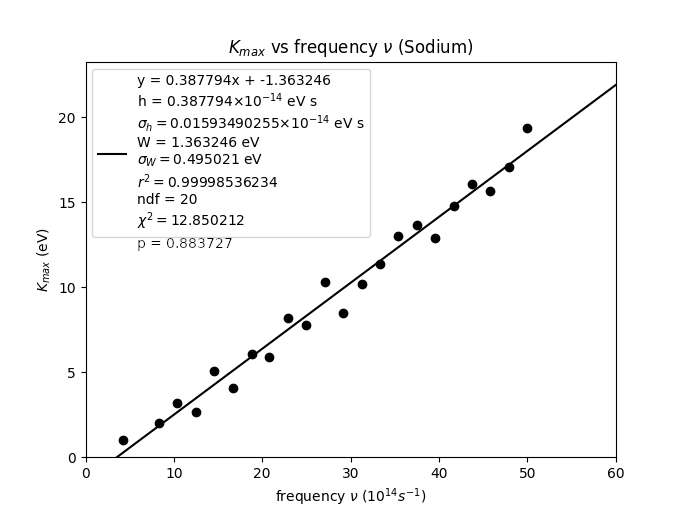
\includegraphics[width=\textwidth]{sodium_plot_1.png}
    \end{minipage}
  \hfill
    \begin{minipage}[b]{0.45\textwidth}
      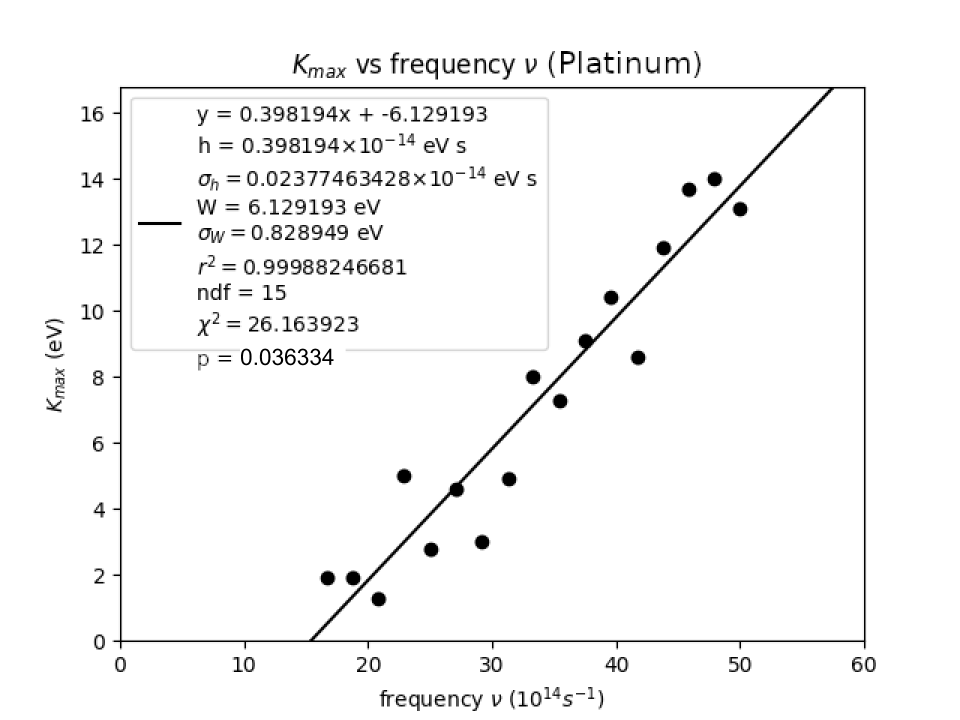
\includegraphics[width=\textwidth]{platinum_plot_1.png}
    \end{minipage}
  \end{figure}
  
  \begin{figure}[ht!]
    \centering
    \begin{minipage}[b]{0.45\textwidth}
      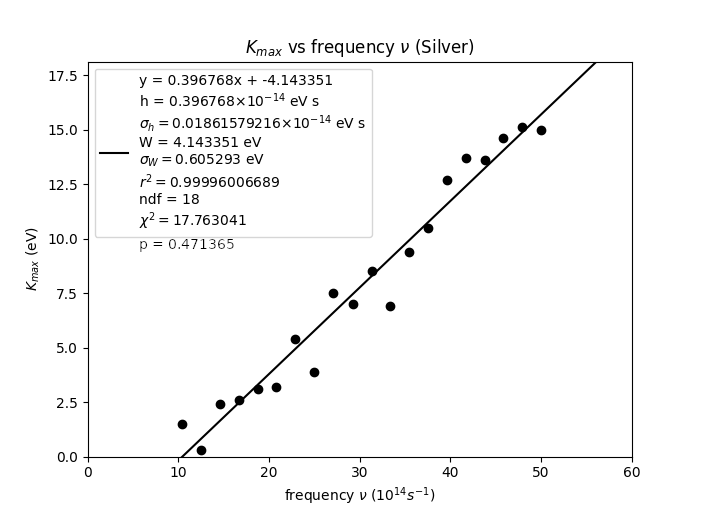
\includegraphics[width=\textwidth]{silver_plot_1.png}
    \end{minipage}
  \hfill
    \begin{minipage}[b]{0.45\textwidth}
      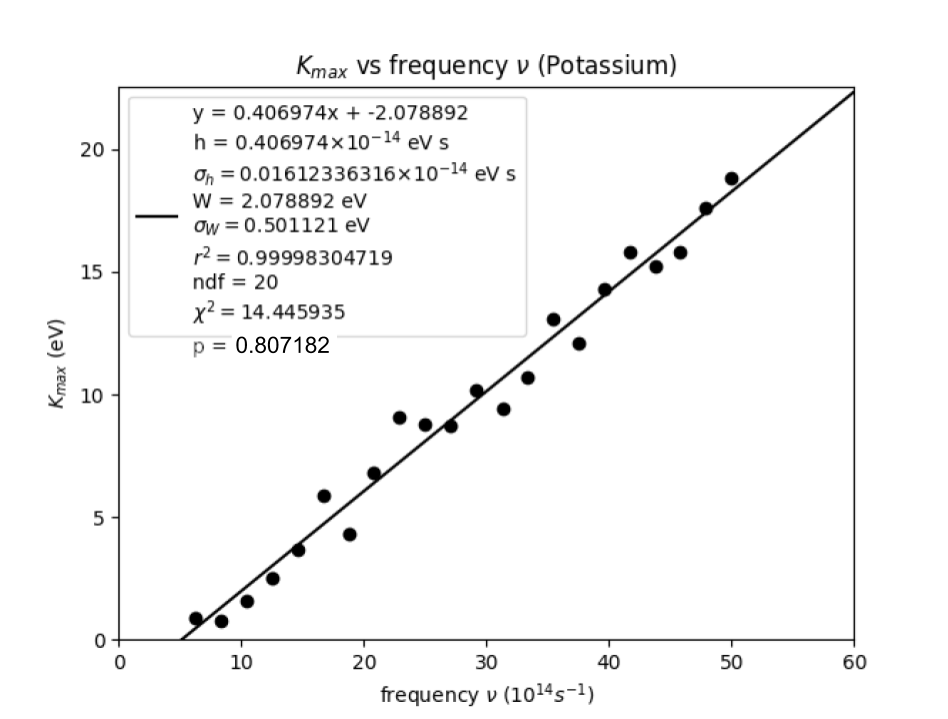
\includegraphics[width=\textwidth]{potassium_plot_1.png}
    \end{minipage}
  \end{figure}

  \begin{figure}[ht!]
    \centering
    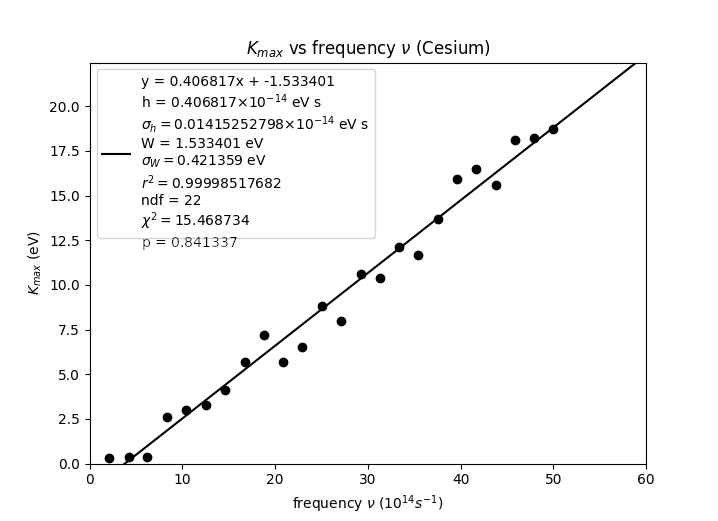
\includegraphics[scale=0.45]{cesium_plot_1.png}
  \end{figure}
  
  \pagebreak
  % ----------------------------------------------------------

  % ------------ table of results for each metal -------------
  \begin{table}[ht]
    \begin{tabular}{|l|l|l|l|l|l|l|}
      \hline
      Metal & $W$ (eV) & $\sigma_W$ (eV) & $W_{true}$ (eV) & $h$ (eV s) & $\sigma_h$ (eV s) & $\chi^2$ \\ \hline
      Sodium (Na) & 1.363246 & 0.495021 & 2.3 & $0.387794 \times 10^{-14}$ & $0.015935\times 10^{-14}$ & 12.850212 \\ \hline
      Platinum (Pt) & 6.129193 & 0.828949 & 6.4 & $0.398194 \times 10^{-14}$ & $0.023775\times 10^{-14}$ & 26.163923 \\ \hline
      Silver (Ag) & 4.143351 & 0.605293 & 4.7 & $0.396768 \times 10^{-14}$ & $0.018616\times 10^{-14}$ & 17.763041 \\ \hline
      Potassium (K) & 2.078892 & 0.501121 & 2.2 & $0.406974 \times 10^{-14}$ & $0.016123\times 10^{-14}$ & 14.445935 \\ \hline
      Cesium (Cs) & 1.533401 & 0.421359 & 1.9 & $0.406817 \times 10^{-14}$ & $0.014153\times 10^{-14}$ & 15.468734 \\ \hline
    \end{tabular}
    \caption{For the work functions $W$ and their uncertainties $\sigma_W$, and for the Planck's constant $h$ and its uncertainty $\sigma_h$, I used the linear regression models in the program ``kmax-vs-nu-linreg.py'' and its forks. For the p-value, I calculated it from the online calculator https://www.socscistatistics.com/pvalues/normaldistribution.aspx, with the f-value input as the ``z-score'' and the the two-tailed hypothesis option. Significance level is $\alpha = 0.5$.}
  \end{table}
  % ----------------------------------------------------------

  % ----------------- comparison of W values -----------------
\item Comparing $W$ values
  \begin{itemize}
  \item For sodium, I obtained a work function of $W_{exp}=1.373246\pm 0.495021$ eV, and its actual work function is $W_{true}=2.3$ eV. Its f-value is therefore
    \begin{align*}
      f &= \frac{W_{exp}-W_{true}}{\sigma_{W_{exp}}^2 + \sigma_{W_{true}}^2} \\
      &= \frac{1.363246-2.3}{0.495021^2+0^2} \\
      &= -3.822771,
    \end{align*}
    which corresponds to a p-value of 0.000132. With a significance level of $\alpha = 0.05$, we have $p < \alpha$, so  my work function for sodium is \textbf{not} in agreement with the actual work function.
    
  \item For platinum, I obtained a work function of $W_{exp}=6.129193\pm 0.828949$ eV, and its actual work function is $W_{true}=6.4$ eV. Its f-value is therefore
    \begin{align*}
      f &= \frac{W_{exp}-W_{true}}{\sigma_{W_{exp}}^2 + \sigma_{W_{true}}^2} \\
      &= \frac{6.129193-6.4}{0.828949^2+0^2} \\
      &= -0.394098,
    \end{align*}
    which corresponds to a p-value of 0.693581. With a significance level of $\alpha = 0.05$, we have $p > \alpha$, so  my work function for platinum is in agreement with the actual work function.

  \item For silver, I obtained a work function of $W_{exp}=4.143351\pm 0.605293$ eV, and its actual work function is $W_{true}=4.7$ eV. Its f-value is therefore
    \begin{align*}
      f &= \frac{W_{exp}-W_{true}}{\sigma_{W_{exp}}^2 + \sigma_{W_{true}}^2} \\
      &= \frac{4.143351-4.7}{0.605293^2+0^2} \\
      &= -1.519323,
    \end{align*}
    which corresponds to a p-value of 0.128762. With a significance level of $\alpha = 0.05$, we have $p > \alpha$, so  my work function for silver is in agreement with the actual work function.

  \item For potassium, I obtained a work function of $W_{exp}=2.078892\pm 0.501121$ eV, and its actual work function is $W_{true}=2.2$ eV. Its f-value is therefore
    \begin{align*}
      f &= \frac{W_{exp}-W_{true}}{\sigma_{W_{exp}}^2 + \sigma_{W_{true}}^2} \\
      &= \frac{2.078892-2.2}{0.501121^2+0^2} \\
      &= -0.482267,
    \end{align*}
    which corresponds to a p-value of 0.629806. With a significance level of $\alpha = 0.05$, we have $p > \alpha$, so  my work function for potassium is in agreement with the actual work function.
    
  \item For cesium, I obtained a work function of $W_{exp}=1.533401\pm 0.421359$ eV, and its actual work function is $W_{true}=1.9$ eV. Its f-value is therefore
    \begin{align*}
      f &= \frac{W_{exp}-W_{true}}{\sigma_{W_{exp}}^2 + \sigma_{W_{true}}^2} \\
      &= \frac{1.533401-1.9}{0.421359^2+0^2} \\
      &= -2.064842,
    \end{align*}
    which corresponds to a p-value of .038923. With a significance level of $\alpha = 0.05$, we have $p < \alpha$, so  my work function for cesium is \textbf{not} in agreement with the actual work function.
  \end{itemize}
  % ----------------------------------------------------------
  
  % ------------- table of f values and p values -------------
  \begin{table}[ht!]
    \begin{tabular}{|l|l|l|l|l|l|l|}
      \hline
      Metal         & $W$ (eV) & $\sigma_W$ (eV) & $W_{true}$ & f-statistic & p-value  & In agreement? \\ \hline
      Sodium (Na)   & 1.363246 & 0.495021        & 2.3 & -3.822771   & 0.000132 & No \\ \hline
      Platinum (Pt) & 6.129193 & 0.828949        & 6.4 & -0.394098   & 0.693581 & Yes \\ \hline
      Silver (Ag)   & 4.143351 & 0.605293        & 4.7 & -1.519323   & 0.128762 & Yes \\ \hline
      Potassium (K) & 2.078892 & 0.501121        & 2.2 & -0.482267   & 0.629806 & Yes \\ \hline
      Cesium (Cs)   & 1.533401 & 0.421359        & 1.9 & -2.064842   & 0.038923 & No \\ \hline
    \end{tabular}
  \end{table}


\end{itemize}

% -------------------------------------------------------------

\section{Calculating and evaluating Planck's constant $h$}

% Table of h values
\begin{table}[ht]
\begin{tabular}{|l|l|l|}
\hline
Metal         & $h$ (eV)                 & $\sigma_h$ (eV)          \\ \hline
Sodium (Na)   & $0.387794\times10^{-14}$ & $0.015935\times10^{-14}$ \\ \hline
Platinum (Pt) & $0.398194\times10^{-14}$ & $0.023775\times10^{-14}$ \\ \hline
Silver (Ag)   & $0.396768\times10^{-14}$ & $0.018616\times10^{-14}$ \\ \hline
Potassium (K) & $0.406974\times10^{-14}$ & $0.016123\times10^{-14}$ \\ \hline
Cesium (Cs)   & $0.406817\times10^{-14}$ & $0.014153\times10^{-14}$ \\ \hline
\end{tabular}
\end{table}

% Calculating h_best
We calculate the best value of Planck's constant, $h_{best}$, using the program h-calc.py. The program uses the following formula:
\begin{align*}
  h &= \frac{\sum_{i=1}^{N}\left(\frac{h_i}{\sigma_{h_i}^2}\right)}{\sum_{i=1}^{N}\left(\frac{1}{\sigma_{h_i}^2}\right)} \\
  h &= 0.400016\times 10^{-14} \text{ eV s}
\end{align*}
We calculate the variance of the best value using h-calc.py, using the following formula:
\begin{align*}
  \sigma_h &= \frac{1}{\sum_{i=1}^{N}\left(\frac{1}{\sigma_{h_i}^2}\right)} \\
  \sigma_h &= 0.007574\times 10^{-14} \text{ eV s}
\end{align*}
Therefore, our best value of $h$ is:
\begin{equation*}\boxed{h_{best} = (0.4000155025 \pm 0.0075740073) \times 10^{-14} \text{ eV s}}\end{equation*}

% Evaluating the fit of h_best
With a true value Planck's constant of $h_{true} = 0.4135667696\times 10^{-14}$ eV s, we calculate f:
\begin{align*}
  f &= \frac{h_{best}-h_{true}}{\sigma_{h_{best}}^2 + \sigma_{h_{true}}^2} \\
  f &= \frac{0.4000155025-0.4135667696}{0.0075740073^2 + 0^2} \\
  f &= -236.226
\end{align*}
Using the calculator www.socscistatistics.com/pvalues/normaldistribution.aspx, we obtain a p-value of approximately 0. At an $\alpha=0.05$ significance level, we have $p<\alpha$, so our value of Planck's constant $h_{best}$ does not agree with the true value $h_{true}$.

% Table of f and p values for h
\begin{table}[ht]
\begin{tabular}{|l|l|l|l|l|}
\hline
$h_{best}$ (eV s) & $\sigma_{h_{best}}$ (eV s) & $h_{true}$ (eV s) & f-statistic & p-value \\ \hline
0.4000155025      & 0.0075740073               & 0.4135667696      & -236.226    & 0       \\ \hline
\end{tabular}
\end{table}

% --------------------------------------------------------
% -------------------- Conclusion ------------------------
% --------------------------------------------------------

\section{Conclusion}

\subsection{$K_{max}$ vs $\nu$ linear regression}
\begin{itemize}
\item Overall, every metal's $K_{max}$ vs $\nu$ plot has a linear model that is a good fit. Sodium has p=0.884, platinum has p=0.036, silver has p=0.471, potassium has p=0.807, cesium has p=0.841. At a significance level of $\alpha = 0.05$, platinum has $p<\alpha$ and thus its linear model is not a good fit for data. The other metals all have $p > \alpha$ and hence their linear models are a good fit for their data.
\end{itemize}


\subsection{W}
\begin{itemize}
\item For the metals sodium and cesium, the calculated value of work function $W$ does not agree with the true value of work function $W_{true}$. Sodium has an f-statistic of -3.822771 and cesium has an f-statistic of -2.064842, indicating that both metals' work functions are lower than the their true values. Sodium has a p-value of 0.000132 and cesium has a p-value of 0.038923, both of which are less than the $\alpha = 0.05$ significance level. This lack of agreement in results may be due to physical properties of the metal making it difficult to masure the maximum kinetic energy $K_{max}$ of the ejected electrons, as sodium and cesium are both Group I metals. The lone valence electron is ejected easily, leading to a large uncertainty in the maximum kinetic energy of the ejected electron. It is also possible that the measuring instrument was calibrated incorrectly for sodium and cesium, leading to measured $K_{max}$ values that were systematically too low.
\item For the metals platinum, silver, and potassium, $W$ agrees with $W_{true}$. Platinum has an f-statistic of -0.394098 and a p-value of 0.693581, silver has an f-statistic of -1.519323 and a p-value of 0.128762, potassium has an f-statistic of -0.482267 and a p-value of 0.038923. All p-values are less than the significance level of $\alpha = 0.05$.
\item All f-statistics were negative, indicating that our measured work functions $W$ were systenatically lower than the actual work functions. However, this experiment did not account for energy lost as the ejected electron hit the detector device. It is also possible that the detector was calibrated so that it made measurements lower than their actual values.
\item In future experiments, I will collect more points for each metal to reduce random error in the calculation of $W$ and $h$ from the linear regression. I will also make sure the device is calibrated correctly, and I will try to use a device that does not lose as much energy when making measurements.
\end{itemize}

\subsection{h}
\begin{itemize}
  \item Our calculated value of Planck's constant $h_{best}$ does not agree with the true value of Planck's constant $h_{true}$. $h_{best}$ has a very low f-statistic of -236.226 and a p-value very close to 0. In other words, our calculated value of Planck's constant is systematically too low. This may be due to systematic error in our measured $K_{max}$ values; the $K_{max}$ tend to be lower than their actual values, and the error scales up as $K_{max}$ increases. For each metal plot, this would result in a slope and hence $h$ that is too low; averaged together, they would produce a $h_{best}$ that is systematically lower than $h_{true}$.
\end{itemize}

In future experiments, I will collect more points for each metal to reduce random error in the calculation of $W$ and $h$ from the linear regression. I will also make sure the device is calibrated correctly, and I will try to use a device that does not lose as much energy when making measurements. That way, the $K_{max}$ values are less likely to be systematically too low, and hence $W$ and $h$ calculations would be closer to their actual values.

\end{document}
